\documentclass[final]{beamer}
\usepackage[scale=1.24]{beamerposter}
\usepackage{graphicx,booktabs,tabularx,algorithm,amsmath}
\usepackage[noend]{algpseudocode}
\usepackage{helvet,tikz}

\usetikzlibrary{arrows,fit,patterns}


\usetheme{confposter}
\setbeamercolor{block title}{fg=Maroon,bg=white}
\setbeamercolor{block body}{fg=black,bg=white}
\setbeamercolor{block alerted title}{fg=white,bg=Maroon!70}
\setbeamercolor{block alerted body}{fg=black,bg=Maroon!10}

\newlength{\sepwid}
\newlength{\onecolwid}
\newlength{\twocolwid}
\newlength{\threecolwid}
\setlength{\paperwidth}{48in}
\setlength{\paperheight}{48in}
\setlength{\sepwid}{0.024\paperwidth}
\setlength{\onecolwid}{0.22\paperwidth}
\setlength{\twocolwid}{0.464\paperwidth}
\setlength{\threecolwid}{0.708\paperwidth}
\setlength{\topmargin}{-0.5in}
\newcolumntype{Y}{>{\centering\arraybackslash}X}


\title{Fido: A Universal Robot Control System Using\\Reinforcement Learning with Limited Feedback}
\author{\LARGE Joshua Gruenstein \and Michael Truell}
\institute{\mbox{}}

\begin{document}

\addtobeamertemplate{block end}{}{\vspace*{2ex}}
\addtobeamertemplate{block alerted end}{}{\vspace*{2ex}}
\setlength{\belowcaptionskip}{2ex}
\setlength\belowdisplayshortskip{2ex}

\begin{frame}[t]
\begin{columns}[t]

\begin{column}{\sepwid}\end{column}
\begin{column}{\onecolwid}

	\begin{alertblock}{Control System Objectives}
		Fido was created to fulfill the following goals:
		\begin{itemize}
			\item \textbf{Trainability}: Allow both human and autonomous training and retraining rather than programming
			\item \textbf{Universality}: Run on any robot and perform any task, even without prior knowledge of the host
			\item \textbf{Performance}: Require few learning iterations and low latency for quick and efficient training
		\end{itemize}
		To achieve this we developed a novel machine learning algorithm utilizing wire-fitted Q-Learning with a neural network, a probabilistic action selection model, and history sampling.  The control system could be trained at a rate \textbf{3 times} the industry standard, allowing practicality over traditional pre-programmed control systems.
	\end{alertblock}

	\begin{block}{System Overview}
		\begin{figure}
			\centering
			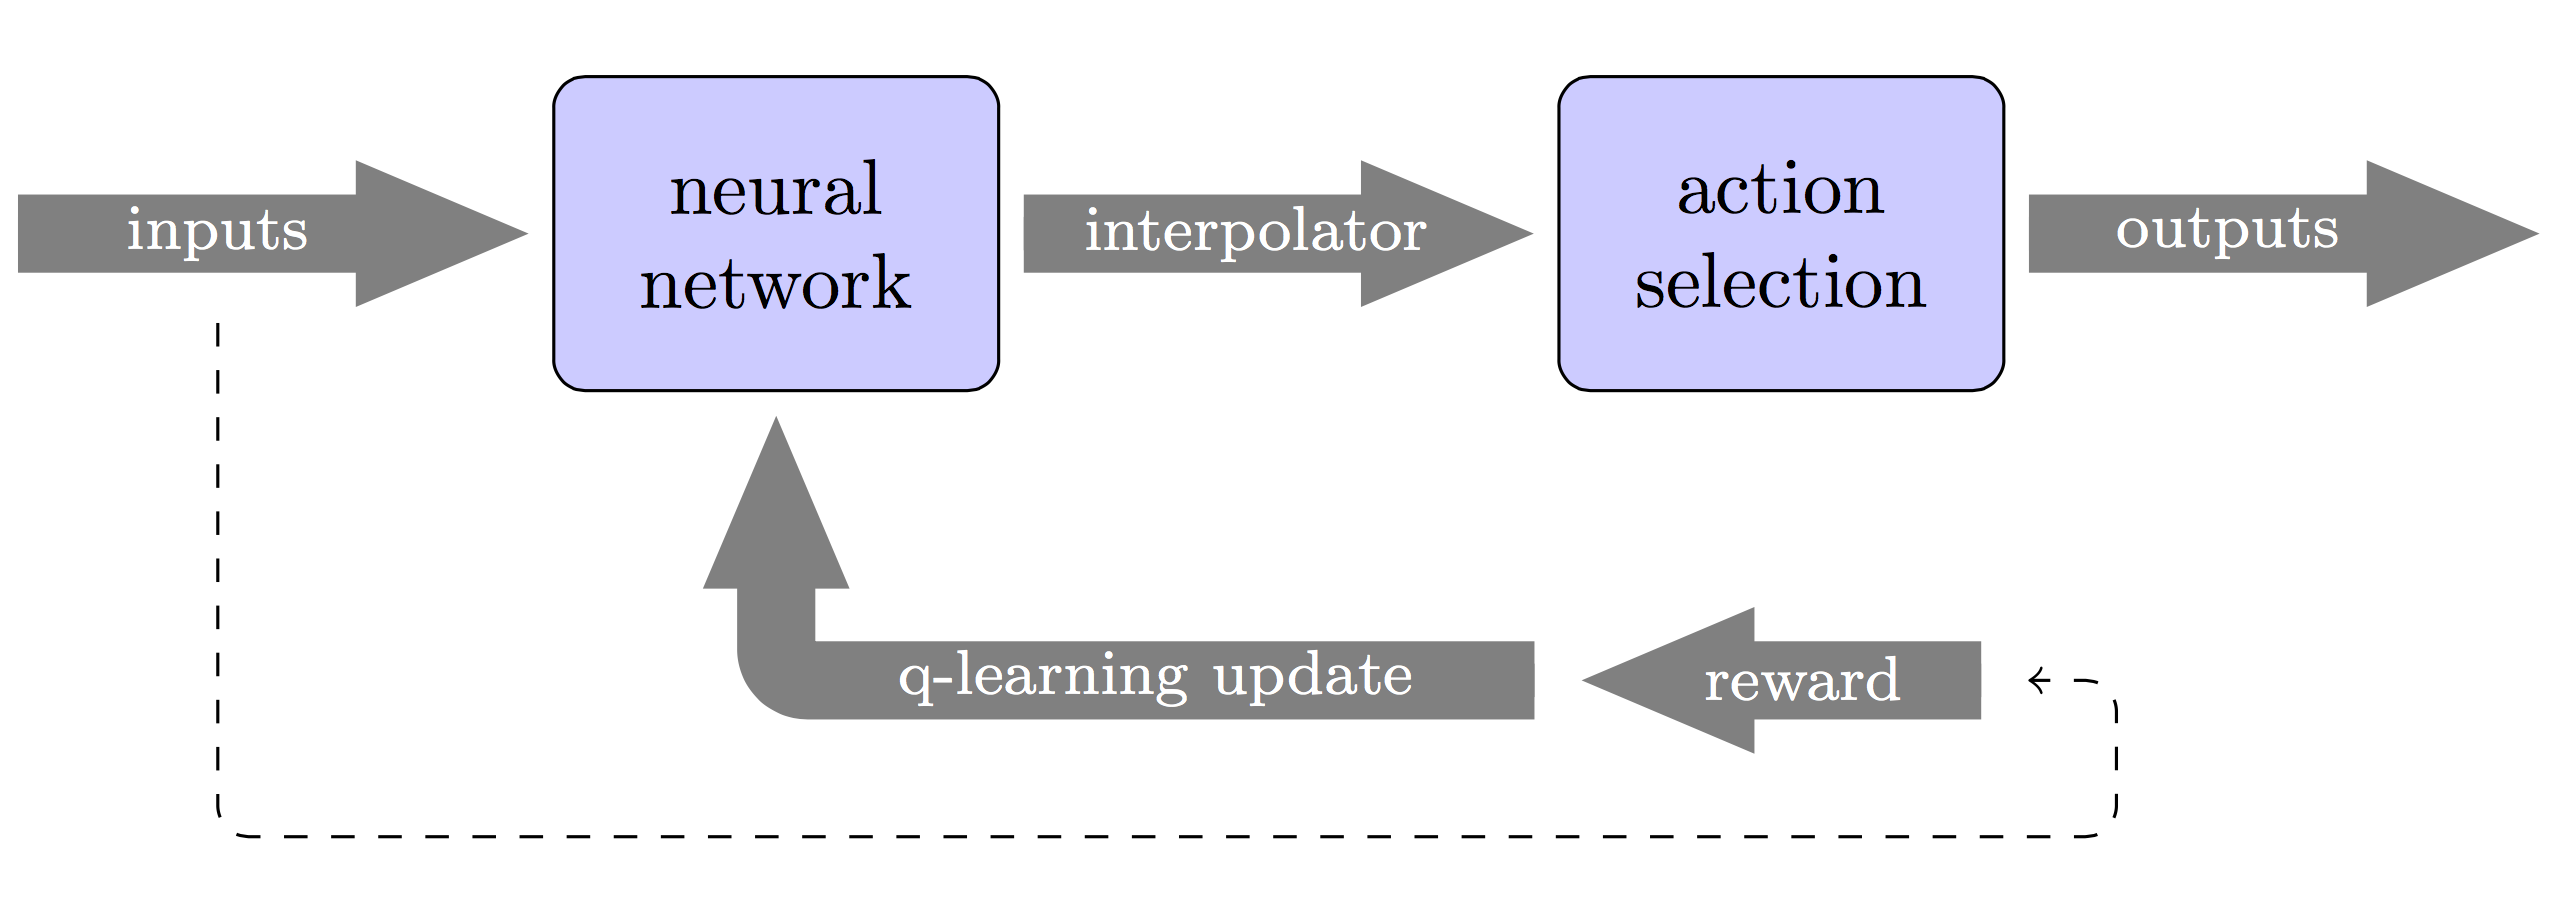
\includegraphics[width=\linewidth]{Figures/diagramRendered.png}
			\caption{Control System Diagram}
		\end{figure}
		\vspace{-1cm}


		\begin{algorithm}
		\caption{Fido Control System}\label{euclid}
		\begin{algorithmic}[1]
			\State Initial empty replay memory $M$
			\State Initial neural network with random weights
			\State Uncertainty value $u \gets \infty$

			\While{$true$}
			  \State Observe state $s_t$
			  \State Feed model $s$ and generate continuous function $r(a)$ of action versus reward
			  \State Select action $a_t$ with expected reward $r_t^*$ using a Softmax action selection policy with temperature $T \propto u$ and the generated $r(a)$ function.

			  \State Execute action $a_t$ and observe reward $r_t$ and new state $s_{t+1}$

			  \State Store ($s_t$, $a_t$, $r_t$, $s_{t+1}$) in $M$

			  \State $u \propto (r_t-r_t^*)^2$

			  \State Sample $n \propto {1/u}$ experiences $e$ giving weight to newer experiences.
			  \State Perform SPSA search on model architectures with cost function as error in predicting $e$ when trained on $e$ using SGD and Adadelta
			  \State Update current model with result of SPSA search
			\EndWhile
		\end{algorithmic}
		\end{algorithm}

		From a macro perspective, Fido can be viewed as a ``black box'' system, where a set of inputs (such as sensors) go in and a set of outputs (actions) go out.  Fido's goal is to maximize given reward by altering its behavior.  The system operates through the following steps:

		\begin{enumerate}
			\item Sensor values are fed to a neural network.
			\item The neural network outputs data points, each is an action and its expected reward.
			\item A wire-fitted least squares interpolator creates a continuous function of action to expected reward using these data points.
			\item An action is chosen using an Softmax selection policy that dynamically adjusts Fido's exploration level as its confidence level changes.
			\item After receiving reward, the neural network is trained to output a new set of data points using Adadelta for gradient descent. Dynamic sizing of the neural network and history sampling are employed to improve neural network performance.
		\end{enumerate}
	\end{block}

\end{column}

\begin{column}{\sepwid}\end{column}

\begin{column}{\twocolwid}

\vspace{-1.65cm}

\begin{columns}[t,totalwidth=\twocolwid]

	\begin{column}{\onecolwid}
		\begin{block}{Reinforcement Learning}
			\begin{itemize}
				\item \textbf{Q-Learning:} A popular reinforcement learning algorithm that develops a function that intakes a state-action pair and outputs expected utility
				\begin{itemize}
					\item However, the Q-function is ordinarily modeled by storing state-action pairs in a table, but this is impractical for large state spaces
					\item A function approximator such as \textbf{Artificial Neural Networks} can be used to model the Q-function instead
				\end{itemize}
				\item Additionally, with regular Q-Learning no relation is made between similar states or actions
				\begin{itemize}
					\item Can be optimized by coupling a wire-fitted interpolator with the neural network (\textbf{Wire-Fitted Q-Learning})
				\end{itemize}

				\item Complete solution: neural network is given sensor values and outputs data points on a graph of possible action vs expected utility, which are interpolated and used to generate a continuous function of action to expected reward.
			\end{itemize}
			\vspace{-1.25cm}
		\end{block}
		\begin{block}{Action Selection}
			\begin{itemize}
				\item Cannot just perform the action with the greatest expected utility: must ``explore'' to be trainable and re-trainable
				\begin{itemize}
					\item Use a Softmax Probability Distribution to select an action, temperature constant governs degree of exploration
				\end{itemize}
				\item However cannot just hardcode the exploration level, as Fido should stop exploring if confident in its actions and explore more if it is being retrained
				\begin{itemize}
					\item Can measure confidence using changes in the neural network weight matrix and adjust exploration accordingly
					\item Increases universality by eliminating the need for an expert to determine the optimal exploration level for a given task
				\end{itemize}
			\end{itemize}
		\end{block}
	\end{column}

	\begin{column}{\onecolwid}\begin{block}{Training}

	\begin{figure}
		\centering
		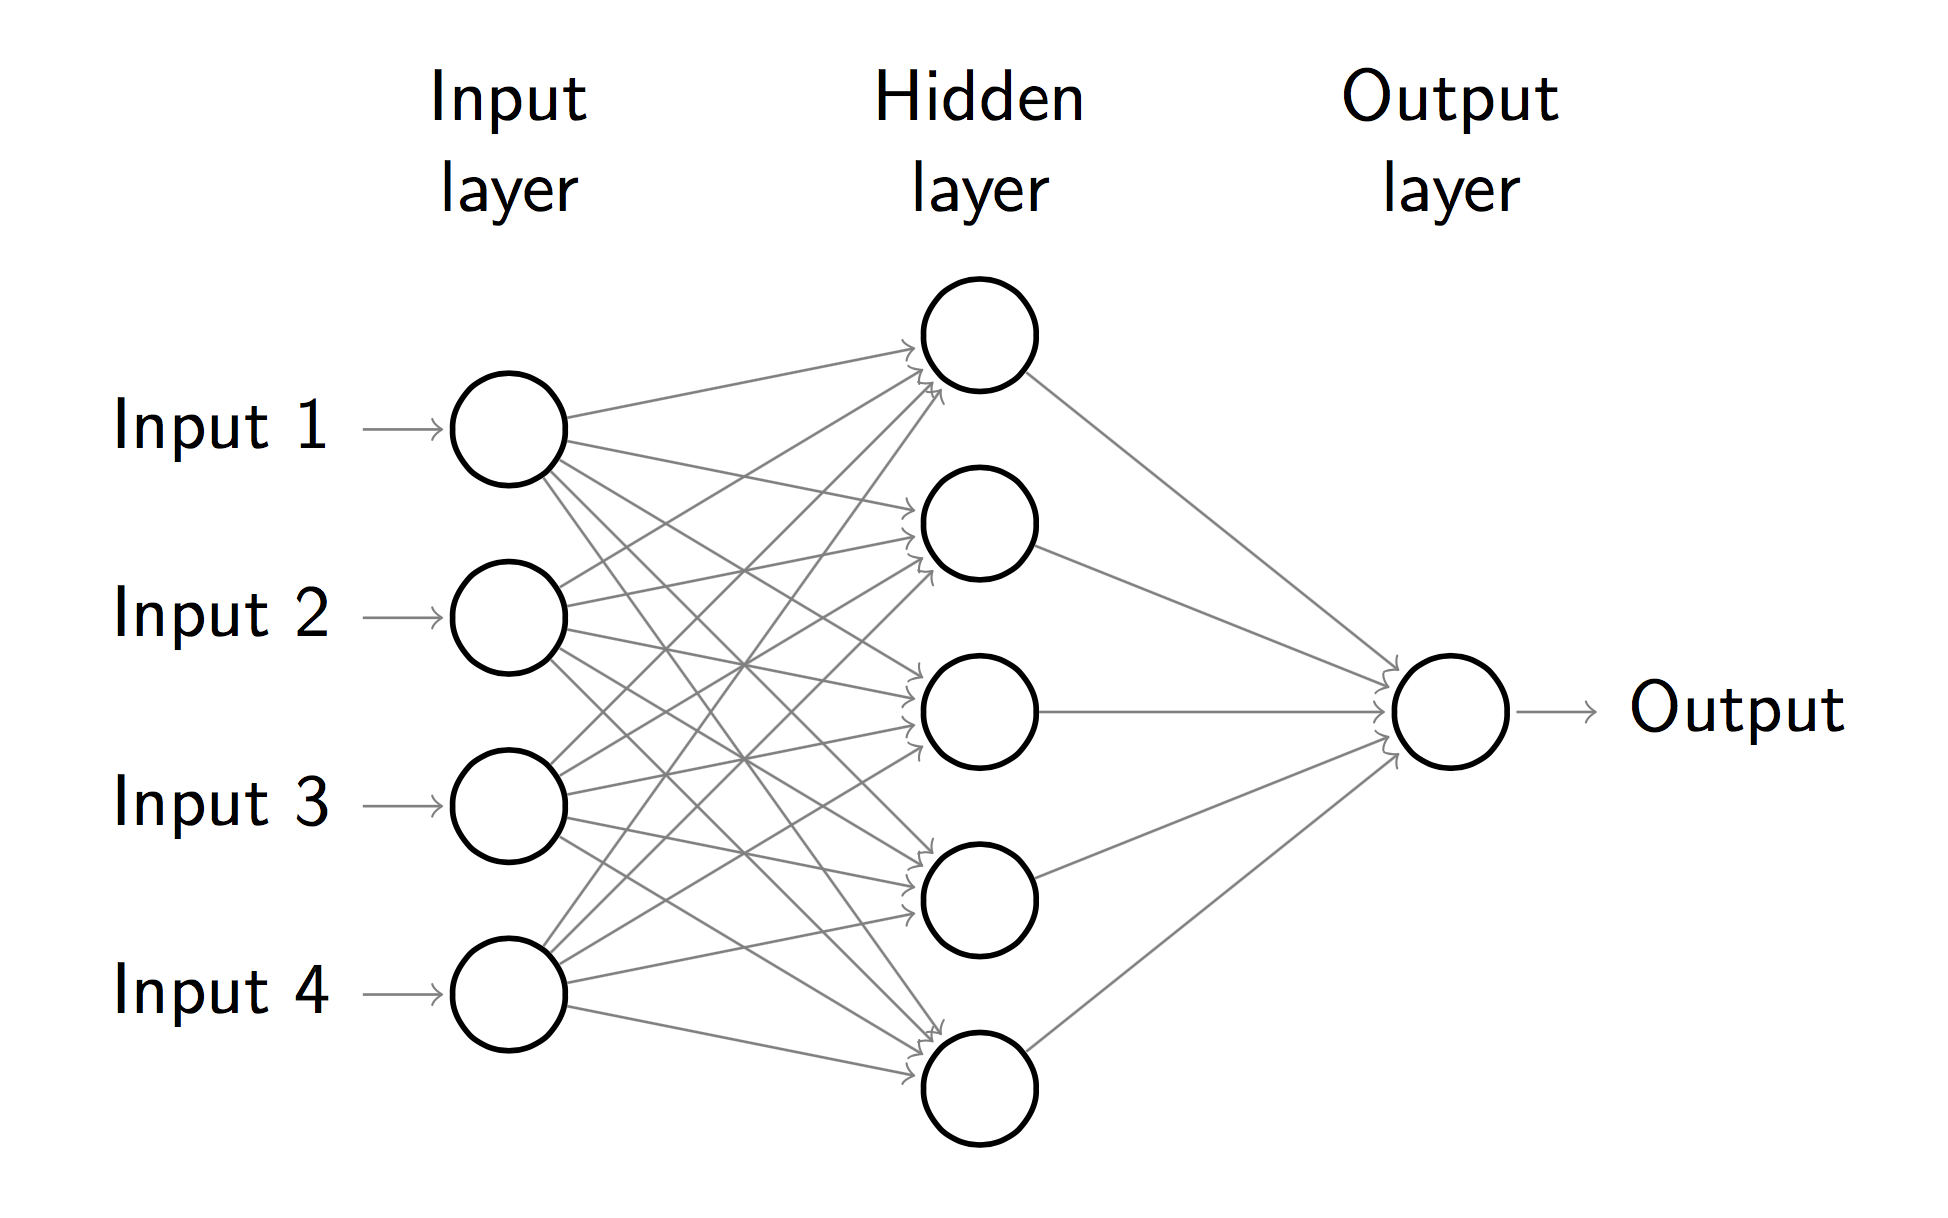
\includegraphics[width=.8\linewidth]{Figures/FeedForwardRendered}
		\caption{Single Output Feed-forward Neural Network}
		\label{fig:feedforward}
	\end{figure}

	\begin{itemize}
		\item After receiving reward, the Fido control system must update its model
		\begin{itemize}
			\item Use Stochastic Gradient Descent to generate a new action to expected reward function for the past state, then train the neural network to output the data points that define this function
		\end{itemize}
		\item However, many neural network training algorithms require a learning rate that depends on the specifics of the task: must be set by an expert in advance
		\begin{itemize}
			\item Can use the new Adadelta training method which dynamically adjusts learning rate, decreases latency, and results in better neural network accuracy
		\end{itemize}
		\item The control system uses \textbf{experience replay} to increase performance, randomly training the neural network on some of Fido's past actions every reward iteration while giving greater weight to newer actions.
		\begin{itemize}
			\item Drastically decreases learning iterations
		\end{itemize}
		\item Additionally, different tasks have different optimal neural network architectures. For example, larger networks are more suited for complicated tasks
		\begin{itemize}
			\item Fido efficiently grows and prunes its neural network using neuron sensitivity approximations gathered from fluctuations in the network's weights.
		\end{itemize}
	\end{itemize}

\end{block}\end{column}

\end{columns}


	\begin{block}{Results}
		Results were gathered both from simulation and hardware for a variety of tasks.    Gathered data for each task included the number of learning iterations, or how many pieces of reward it took for Fido to master the task, action selection time, and training time, or latency in updating Fido's model.
		\begin{table}[ht]
			\centering
			\caption {Fido Results in Simulation (400 trials per task)} \label{tab:simresults}
			\begin{tabularx}{.9\textwidth}{l||Y|Y|Y}
				\toprule
				Task        & Learning Iterations & Action Selection (ms) & Training Time (ms) \\ \midrule
				Flash       & 6                   & 0.                    & 6                  \\
				Float to Point       & 14         & 1                     & 6                  \\
				Drive to Point       & 17         & 1                     & 11                 \\
				Line Following       & 18         & 0.                    & 2                  \\
				Noisy Line Following & 21         & 0.                    & 105                \\
				\bottomrule
			\end{tabularx}
		\end{table}
		\vspace{.5cm}

		\begin{table}[ht]
			\centering
			\caption {Fido Results on Thing One (20 trials per task)} \label{tab:thingoneresults}
			\begin{tabularx}{.9\textwidth}{l||Y|Y|Y}
				\toprule
				Task              & Learning Iterations & Action Selection (ms) & Training Time (ms) \\ \midrule
				Stay Still        & 3                   & 1                    & 43.5                  \\
				Drive to Point    & 18                  & 4                     & 65                  \\
				\bottomrule
			\end{tabularx}
		\end{table}

		\begin{table}[ht]
			\centering
			\caption {Fido Results on Thing Two (20 trials per task)} \label{tab:thingtworesults}
			\begin{tabularx}{.9\textwidth}{l||Y|Y|Y}
				\toprule
				Task              & Learning Iterations & Action Selection (ms) & Training Time (ms) \\ \midrule
				Drive Straight         & 13                   & 2                    & 30                 \\
				Line Following         & 15                  & 21                    & 95                \\
				Fetch                  & 8                  & 1                     & 70                 \\
				Limping Line Following & 6                   & 20                    & 37                 \\
				\bottomrule
			\end{tabularx}
		\end{table}

	\end{block}

\end{column}

\begin{column}{\sepwid}\end{column}

\begin{column}{\onecolwid}
	\begin{block}{Implementation}
		\setlength\parindent{48pt}
		\indent The Fido control system was programmed in C++, with no external dependencies. Two hardware implementations and a simulator were constructed to test Fido's performance.  The first robot utilized a differential drive system and was powered by an Intel Edison embedded GNU/Linux computing platorm, while the second used a holonomic 3x swedish 90 degree wheel arrangment and ran on a \$5 Raspberry Pi Zero.

		\begin{figure}
			\centering
			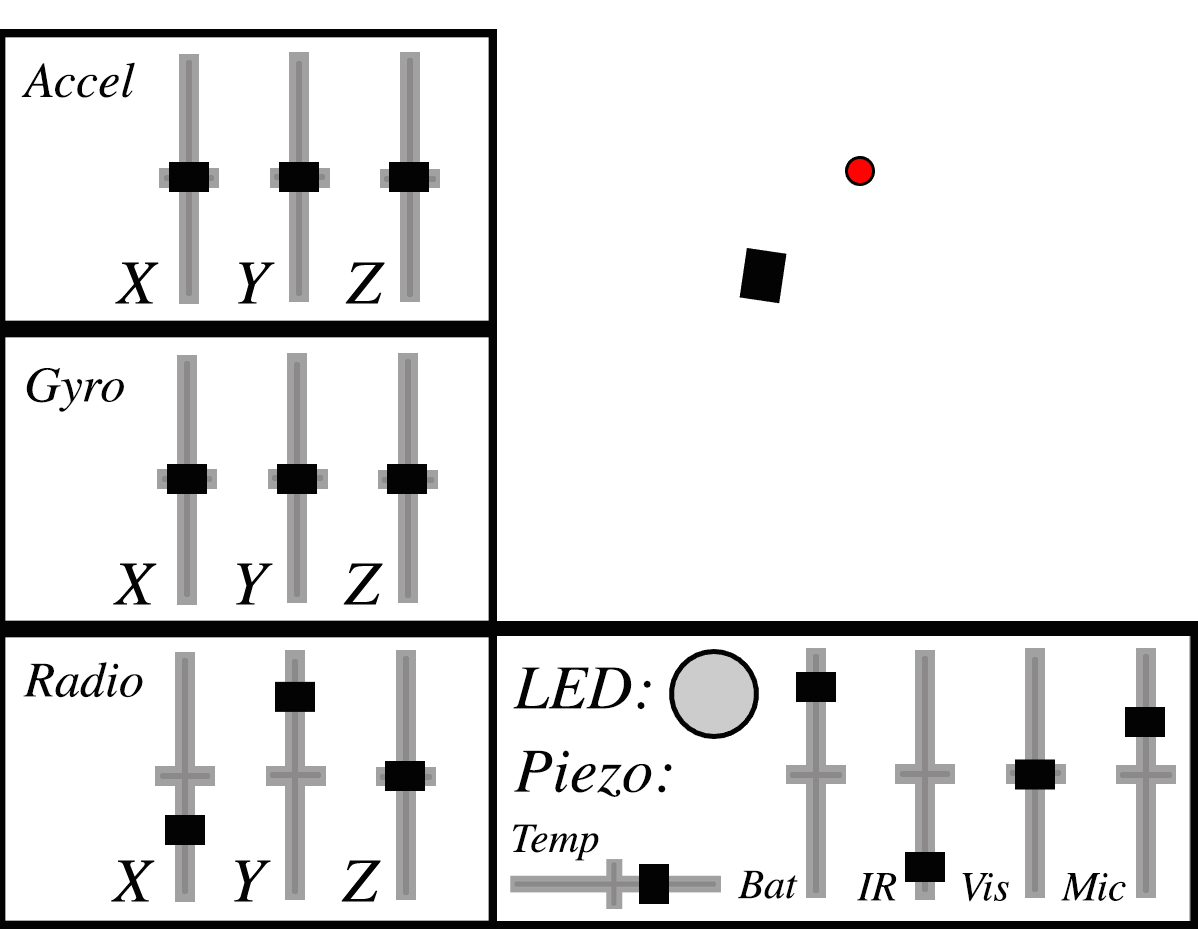
\includegraphics[width=.6\linewidth]{Figures/Screenshot.png}
			\caption{Fido Simulator Graphical User Interface}
		\end{figure}

		\vspace{-0.5in}

		\begin{figure}[ht]
			\centering
			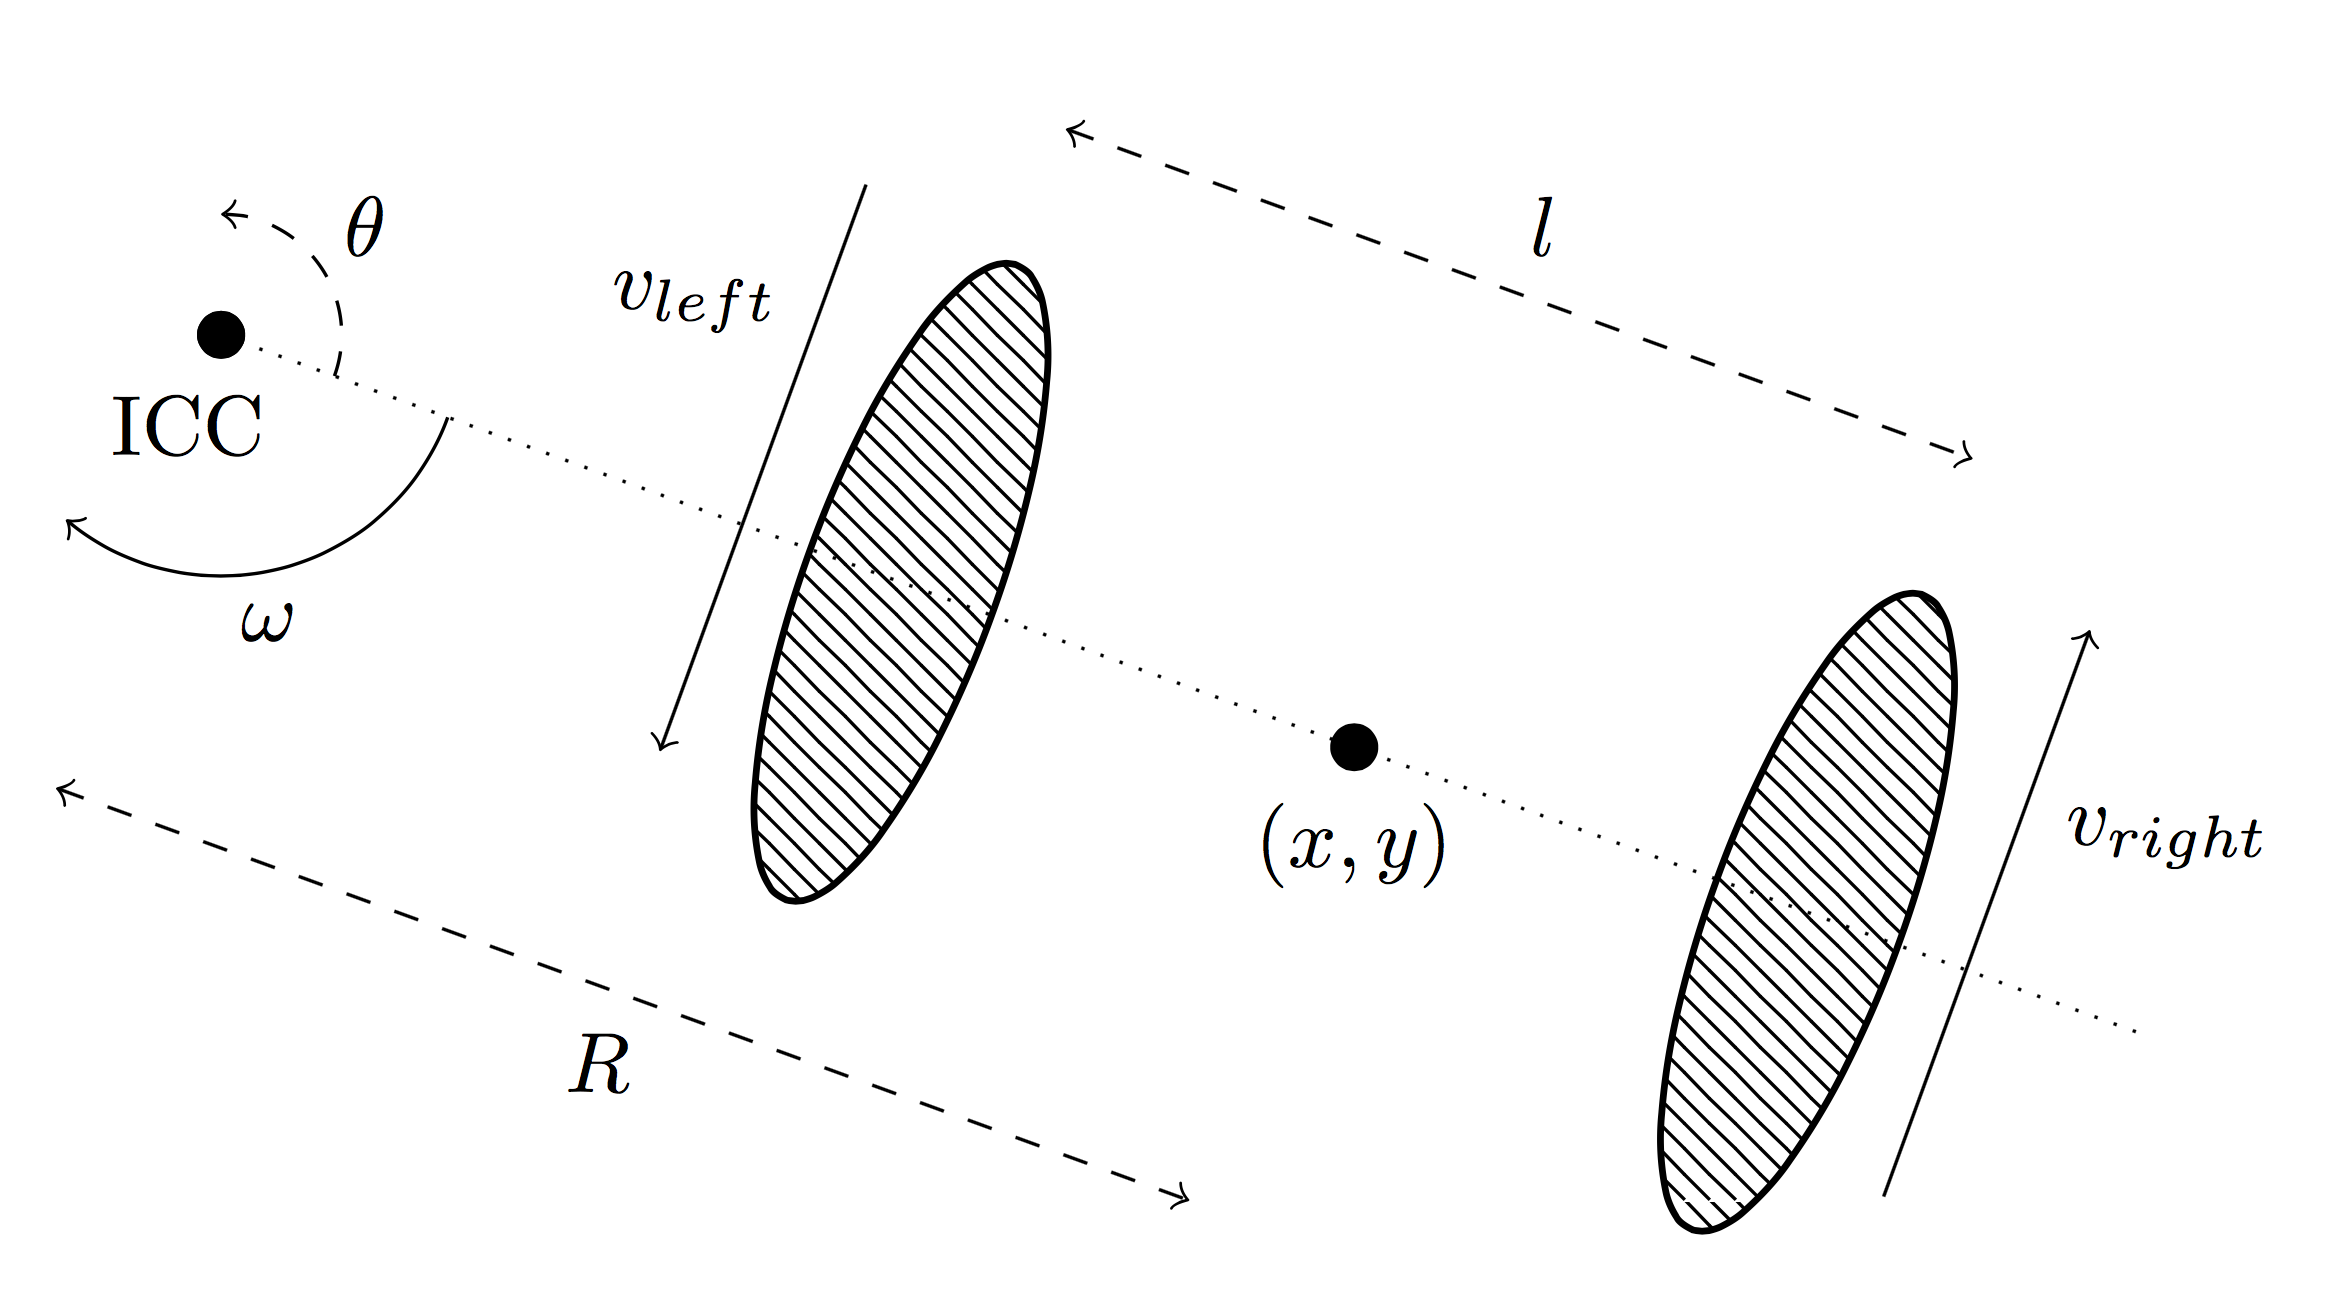
\includegraphics[height=.4\linewidth]{Figures/differentialKinematicsRendered.png}
			\caption{Differential Drive Kinematics}
		\end{figure}

		\vspace{-0.5in}

		\begin{figure}[ht]
			\centering
			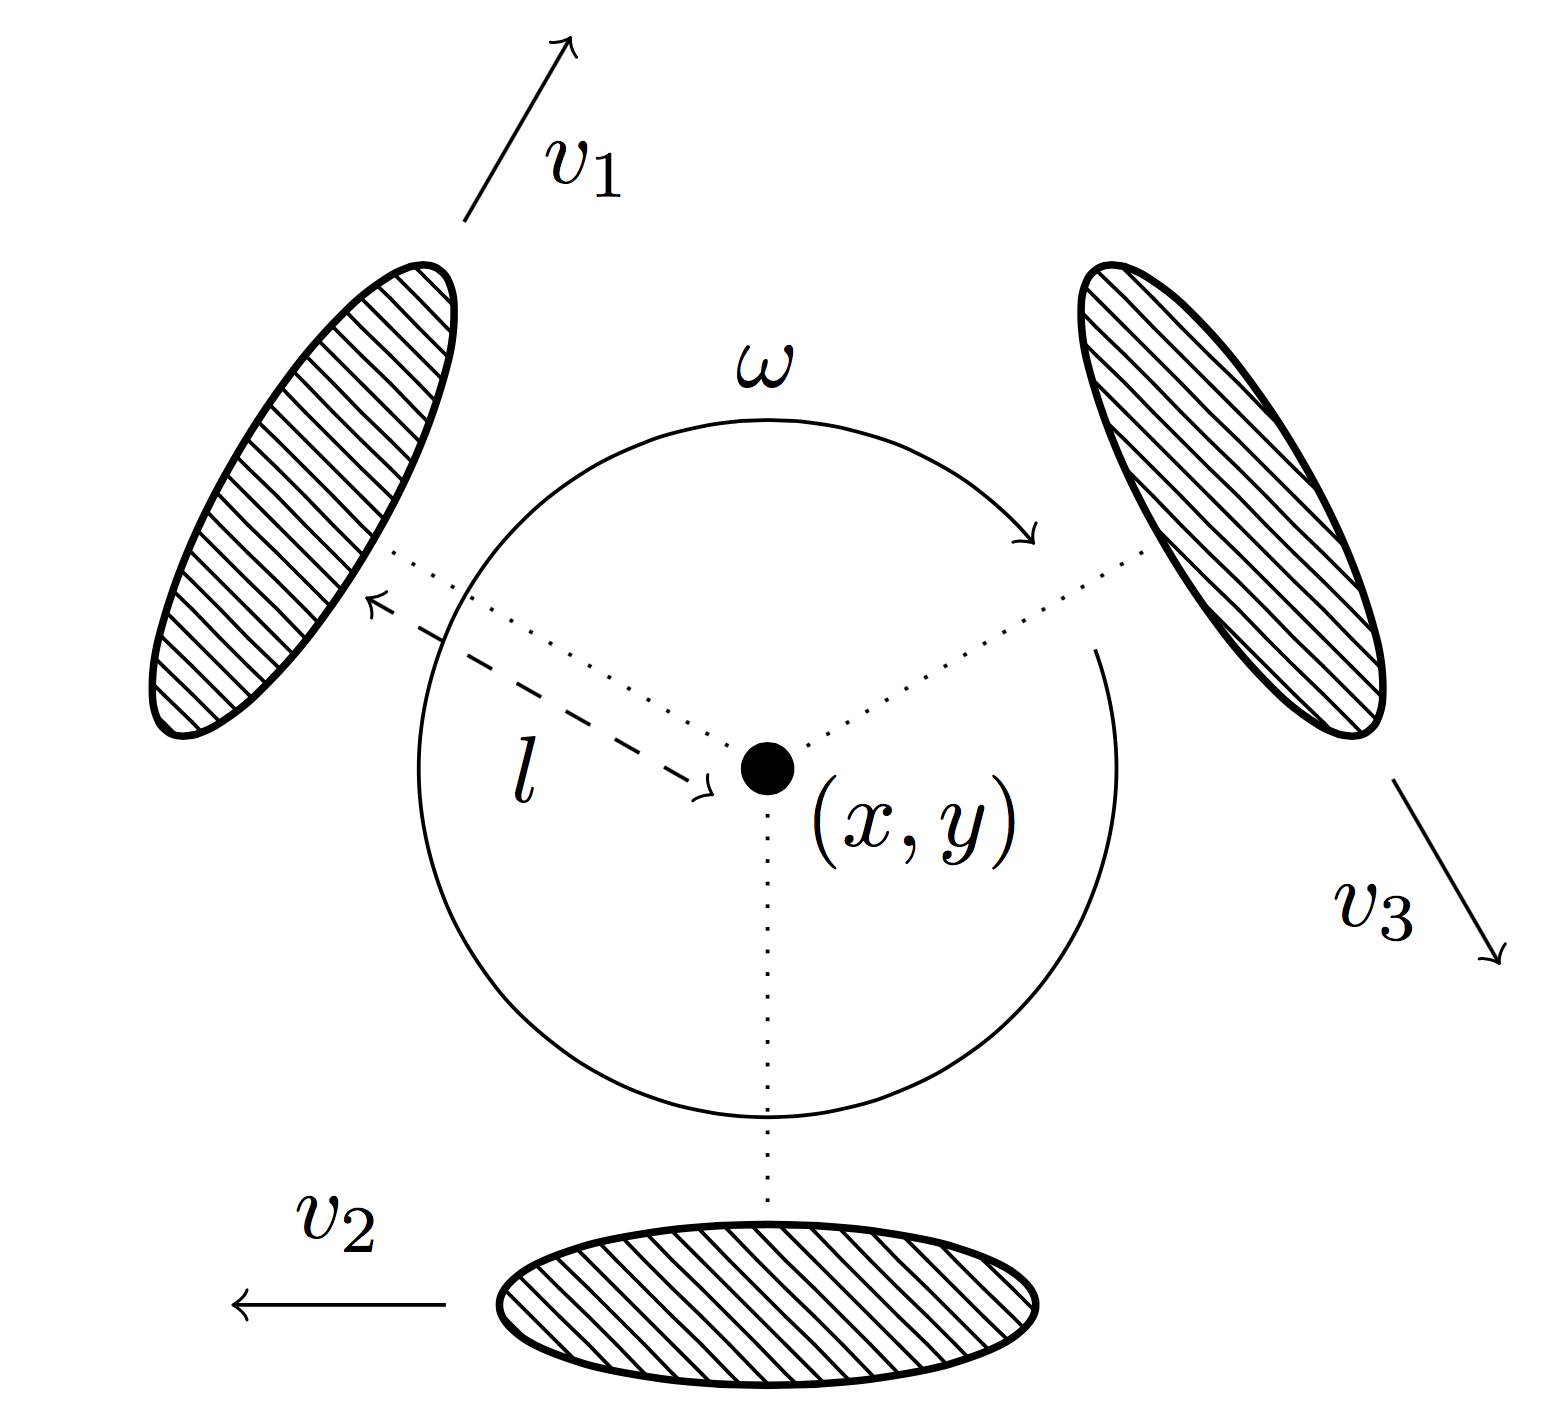
\includegraphics[height=.4\linewidth]{Figures/kiwiKinematicsRendered.png}
			\caption{Holonomic Kiwi Drive Kinematics}
		\end{figure}
	\end{block}

	\begin{block}{Applications}
		Fido provides numerous advantages over traditional procedural-programmed control systems, making it practical for a number of real world applications.  As Fido can be trained and retrained without expert knowledge, it could be useful in making robotics more accessible to consumers and small-buisness owners.  Fido can also be retrained to adapt to new and unexpected circumstances such as malfunctions in the field, an advantageous feature for militiary applications.
	\end{block}

	\begin{block}{Selected References}
		\nocite{*}
		{\fontsize{25}{30}\bibliographystyle{IEEEtran}\bibliography{Poster}\vspace{0.75in}}
	\end{block}

\end{column}

\end{columns}
\end{frame}
\end{document}

%%%%%%%%%%%%%%%%%%%%%%%%%%%%%%%%%%%%%%%%%
% Adapted from "Jacobs Landscape Poster"
% https://teamwork.jacobs-university.de:8443/confluence/display/CoPandBiG/LaTeX+Poster
% License: CC BY-NC-SA 3.0 (http://creativecommons.org/licenses/by-nc-sa/3.0/)
%%%%%%%%%%%%%%%%%%%%%%%%%%%%%%%%%%%%%%%%%
